% !TeX root = ../tesis.tex


\section{Relaciones de Kramers-Kronig}
\label{section:rKK}

El estudio del esparcimiento y la absorción de partículas mediante secciones transversales proporciona una descripción macroscópica de su respuesta óptica. Este enfoque se complementa con una caracterización microscópica del material, representada por su función dieléctrica~$\varepsilon(\omega)$~\cite{KramersKronigRelationsOptical2005}. En el espacio de frecuencias, la función dieléctrica de un material es, en general, una función compleja: su parte real $\varepsilon'(\omega)$ representa la capacidad del material para almacenar energía mediante la polarización eléctrica, mientras que su parte imaginaria $\varepsilon''(\omega)$ describe la disipación o pérdida de energía debida a procesos de absorción \cite{maierPlasmonicsFundamentalsApplications2007b}. Desde un punto de vista físico, $\varepsilon''(\omega)$ se origina en el desfase entre el campo eléctrico incidente y la respuesta inducida de los dipolos del material~\cite{royHilbertTransformBrief2024}. Experimentalmente, a menudo solo se puede realizar la medición directa de una de las dos contribuciones de $\varepsilon(\omega)$. Por ejemplo, técnicas como la espectroscopía de absorción o de transmisión permiten obtener información disipativa, es decir, de $\varepsilon''$ \cite{KramersKronigRelationsOptical2005}. Esta limitación motiva el desarrollo de las relaciones de Kramers-Kronig (KK), las cuales establecen una conexión  entre las partes real e imaginaria de cualquier función óptica lineal compleja \cite{KramersKronigRelationsOptical2005}. La base de las relaciones KK reside en el principio de causalidad \cite{KramersKronigRelationsOptical2005}: la respuesta del sistema no puede preceder temporalmente a la excitación que la genera. En el contexto del esparcimiento de ondas electromagnéticas, esto implica que el campo esparcido no puede existir antes de que la onda incidente alcance el centro de esparcimiento \cite{KramersKronigRelationsOptical2005}. Este principio, junto con la condición de analiticidad\footnote{Una función compleja $f(x+iy)=u(x,y)+i\,v(x,y)$ es analítica si $u$ y $v$ tienen primeras derivadas continuas y satisfacen las ecuaciones de Cauchy-Riemann \cite{arfkenMathematicalMethodsPhysicists2011a}.} de la función óptica en el semiplano superior del plano complejo de frecuencias, garantiza que las partes real e imaginaria de funciones como la susceptibilidad eléctrica, la función dieléctrica, el índice de refracción o la reflectividad no sean independientes. Por el contrario, que estén acopladas a través de una transformada de Hilbert \cite{KramersKronigRelationsOptical2005}. Esto implica que el conocer la respuesta disipativa [$\varepsilon''(\omega)$] en todo el espectro de frecuencias es, en principio, suficiente para determinar de manera unívoca la respuesta óptica asociada al esparcimiento [$\varepsilon'(\omega)$], y viceversa.

En esta sección se considera un material homogéneo e isótropo, caracterizado por una función óptica lineal compleja, en particular la función dieléctrica, definida en un espacio de frecuencias complejo. El objetivo es derivar las relaciones de 
KK asociadas a dicha función. Para ello, se emplean las transformadas de Fourier directa e inversa de los campos $\vb{E}$ y $\vb{D}$, a partir de las cuales se obtiene una expresión para la permitividad eléctrica relativa. Posteriormente, se imponen condiciones de causalidad sobre esta expresión que permiten  garantizar su analiticidad en el semiplano superior del plano complejo de frecuencias y con ello deducir las relaciones de KK.

Las transformadas de Fourier temporales directa e inversa de $\vb{D}$ se definen como~\cite{jacksonClassicalElectrodynamics2021a}
%
\begin{equation}
	\vb{D}(\vb{r},\omega)=\int_{-\infty}^{\infty}\vb{D}(\vb{r},t')e^{i\omega t'}\text{d}t',\;\;\text{y}\;\;\vb{D}(\vb{r},t)=\frac{1}{2\pi}\int_{-\infty}^{\infty}\vb{D}(\vb{r},\omega)e^{-i\omega t}\text{d}\omega,\label{eq:TFD}
\end{equation}
%
respectivamente. Al sustituir la Ec. para $\vb{D}$ en  \eqref{eq:d3_b3} en la transformada de Fourier inversa de las Ecs. \eqref{eq:TFD}, se obtiene
\vspace{-0.5cm}

%
\begin{equation}
	\vb{D}(\vb{r},t)=\frac{1}{2\pi}\int_{-\infty}^{\infty}\varepsilon(\omega)\vb{E}(\vb{r},\omega)e^{-i\omega t}\text{d}\omega,\label{eq:TF_D_intermedia_1}
\end{equation}
%
y al expresar $\vb{E}(\vb{r},\omega)$ mediante su transformada de Fourier, la Ec. \eqref{eq:TF_D_intermedia_1} se reescribe como
%
\begin{align}
	\vb{D}(\vb{r},t)&=\frac{1}{2\pi}\int_{-\infty}^{\infty}\varepsilon(\omega)e^{-i\omega t}\text{d}\omega\int_{-\infty}^{\infty}e^{i\omega t'}\vb{E}(\vb{r},t')\text{d}t',\\
	&=\frac{1}{2\pi}\int_{-\infty}^{\infty}\int_{-\infty}^{\infty}\varepsilon(\omega)\vb{E}(\vb{r},t') e^{i\omega (t-t')} \text{d}\omega \text{d}t',
	\label{eq:TF_D_intermedia_2}
\end{align}
%
donde además se consideró que los órdenes de integración se pueden intercambiar dado que la integración se realiza en el mismo intervalo ($-\infty$, $\infty$). Para imponer las propiedades de causalidad en una única función respuesta $G(\tau)$, con $\tau = t - t'$, donde $t$ es el tiempo de observación y $t'$ todos los demás, se escribe al campo eléctrico como\footnote{Donde se realiza el cambio de variable $\tau = t - t'$ y se emplea la función constante \cite{arfkenMathematicalMethodsPhysicists2011a}
	%
\begin{equation}
	\mathscr{F}[1]=\int_{-\infty}^{\infty}e^{-i\omega\tau}=\delta(\tau),
	\end{equation}
%
con $\delta(\tau)$ la función delta de Dirac, que cumple con $\int_{-\infty}^{\infty}f(\tau)\delta(\tau)\text{d}\tau=f(0)$ \cite{arfkenMathematicalMethodsPhysicists2011a}.
}
\begin{equation}
	\vb{E}(\vb{r},t)=\int_{-\infty}^{\infty}\vb{E}(\vb{r},t-\tau)\delta(\tau)=\frac{1}{2\pi}\int_{-\infty}^{\infty}\int_{-\infty}^{\infty}\vb{E}(\vb{r},t-\tau)e^{-i\omega\tau}\text{d}\omega\text{d}\tau,
\end{equation}
%
con $\delta(\tau)$ la delta de Dirac. Al sumar $\vb{E}(\vb{r},t')-\vb{E}(\vb{r},t')$ y multiplicar por $\varepsilon_0/\varepsilon_0$ a la Ec. \eqref{eq:TF_D_intermedia_2}, simplificando se obtiene
%
\begin{equation}
	\vb{D}(\vb{r},t)=\varepsilon_0\left[\vb{E}(\vb{r},t)+\int_{-\infty}^{\infty}G(\tau)\vb{E}(\vb{r},t-\tau)\text{d}\tau\right],\label{eq:TF_D_final} 
\end{equation}
%
\noindent donde $G(\tau)$ es \cite{jacksonClassicalElectrodynamics2021a}
%
\begin{equation}
	G(\tau)=\frac{1}{2\pi}\int_{-\infty}^{\infty}\left[\frac{\varepsilon(\omega)}{\varepsilon_0}-1\right]e^{-i\omega\tau}\text{d}\omega,
	\label{eq:G_tdependent} 
\end{equation}
%
\noindent con $\varepsilon(\omega)/\varepsilon_0$ la permitividad eléctrica relativa. Al aplicar la transformada de Fourier a la Ec.~\eqref{eq:G_tdependent}, se obtiene una expresión para la permitividad eléctrica relativa
%
\begin{equation}
	\frac{\varepsilon(\omega)}{\varepsilon_0}=1+\int_{-\infty}^{\infty}G(\tau) e^{-i\omega\tau}\text{d}\tau.
	\label{eq:epsrelativa} 
\end{equation}
%
\noindent Las Ecs. \eqref{eq:TF_D_final} y \eqref{eq:G_tdependent} muestran que el campo de desplazamiento eléctrico al tiempo $t$ depende del campo eléctrico en todos los demás tiempos $t'$. A esta característica, se le conoce como la no localidad temporal entre $\vb{D}$ y $\vb{E}$ \cite{jacksonClassicalElectrodynamics2021a}. 
\vspace{0.1cm}

De modo que las Ecs. \eqref{eq:TF_D_final} y \eqref{eq:epsrelativa} sean causales, es necesario imponer condiciones que garanticen que la Ec. \eqref{eq:G_tdependent} se anule para $\tau<0$, lo que se traduce en que al tiempo $t$, únicamente valores del campo eléctrico previos a ese tiempo determinan el vector de desplazamiento eléctrico~\cite{jacksonClassicalElectrodynamics2021a}. De esta forma, las Ecs. \eqref{eq:TF_D_final} y \eqref{eq:epsrelativa} se reescriben como
%
\begin{subequations}%
	\begin{tcolorbox}[
		ams align, breakable]
		\vb{D}(\vb{r},t)&=\varepsilon_0\left[\vb{E}(\vb{r},t)+\int_{0}^{\infty}G(\tau)\vb{E}(\vb{r},t-\tau)\text{d}\tau\right],\\ \label{seq:D_final}
		\frac{\varepsilon(\omega)}{\varepsilon_0}-1&=\int_{0}^{\infty}G(\tau) e^{-i \omega\tau}\text{d}\tau,\label{seq:G}	\end{tcolorbox}
\end{subequations}
%
\noindent donde $\varepsilon(\omega)$ es una función compleja, cuyas partes real e imaginaria se relacionan como $\varepsilon(-\omega)/\varepsilon_0=\varepsilon^*(\omega^*)/\varepsilon_0$.

Dado que $\vb{E}(\vb{r},t)$ y $\vb{D}(\vb{r},t)$ son funciones reales, $G(\tau)$ también lo es. Si se considera a la Ec. \eqref{seq:G} como una representación de $	\varepsilon(\omega')/\varepsilon_0$ en el plano complejo, entonces la Ec. \eqref{seq:G} es analítica en el semiplano superior complejo siempre que $G(\tau)$ sea finita para toda $\tau$ \cite{jacksonClassicalElectrodynamics2021a}. Para que dicha analiticidad se extienda hasta el eje real, es necesario imponer la condición $G(\tau)\rightarrow 0$ cuando $\tau\rightarrow \infty$ \cite{jacksonClassicalElectrodynamics2021a} \footnote{Esto se cumple para dieléctricos; en conductores, en cambio, se tiene que $G(\tau)\rightarrow \sigma/\epsilon_0$ cuando $\tau\rightarrow \infty$~\cite{jacksonClassicalElectrodynamics2021a}. }. Como $\varepsilon(\omega')/\varepsilon_0-1$ es una función analítica en el semiplano superior complejo incluyendo el eje real, la función $	[\varepsilon(\omega')/\varepsilon_0-1]/(\omega'-\omega)$ también lo es, salvo por la singularidad en $\omega'=\omega$. De acuerdo con el teorema integral de Cauchy\footnote{El teorema integral de Cauchy establece que si una función $f(z)$ es analítica dentro y sobre un contorno cerrado $C$, entonces $\oint_C f(z)/(z-z_0)\dd{z}= 0$ \cite{arfkenMathematicalMethodsPhysicists2011a}.}, para un contorno cerrado $C$ que no encierre $\omega_0$ se cumple \cite{arfkenMathematicalMethodsPhysicists2011a}
%
\begin{equation}
	\oint_C \frac{[\varepsilon(\omega')/\varepsilon_0-1]}{\omega'-\omega}\dd{\omega'}= 0.
	\label{eq:Cauchy}
\end{equation}
%
Para determinar el contorno apropiado de modo que se pueda emplear la Ec. \eqref{eq:Cauchy}, se considera a $\omega$ un punto sobre el eje real y a $C$ la unión de cuatro curvas con representaciones paramétricas como se muestra en la Fig. \ref{fig:integration_contour0} y que están dadas por \cite{bohrenAbsorptionScatteringLight2008}
%
\begin{align*}
	C_1&: \; \omega'=\Omega, & -A\leq \Omega \leq \omega-a,\\
	C_2&: \; \omega'=\omega-ae^{-i\Omega}, & 0\leq\Omega\leq\pi,\\
	C_3&: \;\omega'=\Omega, & \omega+a\leq\Omega\leq A,\\
	C_4&: \;\omega'=Ae^{i\Omega}, & 0\leq\Omega\leq \pi.
\end{align*}
%
\begin{figure}[h!]
	\centering
	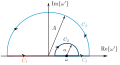
\includegraphics[width=8cm]{../../Figuras/integration.pdf}
	\caption{Contorno de integración $C$ conformado por cuatro curvas.}
	\label{fig:integration_contour0}
\end{figure}
%
Así, la Ec. \eqref{eq:Cauchy} se reescribe como
\begin{align*}
	\int_A^{\omega-a}\frac{[\varepsilon(\Omega)/\varepsilon_0-1]}{\Omega-\omega}\dd{\Omega}&+	\int_{\omega+a}^{A}\frac{[\varepsilon(\Omega)/\varepsilon_0-1])}{\Omega-\omega}\dd{\Omega}+\\
	&+	\int_0^{\pi}\frac{iA\;e^{i\Omega}\; [\varepsilon(A\;e^{i\Omega})/\varepsilon_0-1]}{A\;e^{i\Omega}-\omega}\dd{\Omega}-\int_0^{\pi}i\;[\varepsilon(\omega-ae^{-i\Omega})/\varepsilon_0-1]\dd{\Omega}=0.
\end{align*}
Integrando por partes la Ec. \eqref{seq:G}, se obtiene  
%
\begin{equation*}
	\frac{\varepsilon(\omega)}{\varepsilon_0}-1=\frac{i G^{(0)}(0)}{\omega}-\frac{ G^{(1)}(0)}{\omega^2}+\frac{i G^{(2)}(0)}{\omega^3}+...,
\end{equation*}
%
donde $G^{(i)}(\tau)$ indica la $i$-ésima derivada y donde se empleó que $G(\tau)\rightarrow 0$ cuando $\tau\rightarrow \infty$. Además, dado que $G(\tau)$ es causal, $G(0)=0$; por lo que el primer término se anula al igual que los términos que decaen más rápido que $1/\omega^2$ a frecuencias altas. Con ello, por el lema de Jordan\footnote{El lema de Jordan establece que si una función es continua en un contorno semicircular de radio $R$ centrado en el origen y acotada cuando $R\rightarrow \infty$, entonces la integral sobre el contorno semicircular es 0 \cite{arfkenMathematicalMethodsPhysicists2011a}. } la integral sobre el segmento $C_4$ es \cite{bohrenAbsorptionScatteringLight2008}
%
\begin{equation}
	\int_0^{\pi}i\;[\varepsilon(\omega-ae^{-i\Omega})/\varepsilon_0-1]\dd{\Omega}=0.
\end{equation}
%
 Por otro lado, al considerar el límite de $a\to 0$ y al emplear nuevamente el teorema de Cauchy, la integral sobre el segmento $C_2$ es \cite{jacksonClassicalElectrodynamics2021a} 
 %
 \begin{equation*}
	\int_0^{\pi}i\;[\varepsilon(\omega-ae^{-i\Omega})/\varepsilon_0-1]\dd{\Omega}=i\pi[\varepsilon(\Omega)/\varepsilon_0-1].
 \end{equation*}
 %
 Finalmente, las integrales sobre los segmentos $C_1$ y $C_3$ equivalen a 
%
\begin{equation}
		\int_A^{\omega-a}\frac{[\varepsilon(\Omega)/\varepsilon_0-1]}{\Omega-\omega}\dd{\Omega}+	\int_{\omega+a}^{A}\frac{[\varepsilon(\Omega)/\varepsilon_0-1])}{\Omega-\omega}\dd{\Omega}=\text{PV}\int_{-\infty}^{\infty}\frac{[\varepsilon(\Omega)/\varepsilon_0-1]}{\Omega-\omega} \dd{\Omega},
\end{equation}
%
donde P.V. denota el valor principal de la integral \cite{arfkenMathematicalMethodsPhysicists2011a}. Por lo tanto, se obtiene 
%
\begin{equation}
	\PV{\int_{-\infty}^{\infty}\frac{[\varepsilon(\omega')/\varepsilon_0-1]}{\omega'-\omega} \dd{\omega'}}=i\pi[\varepsilon(\omega')/\varepsilon_0-1].
	\label{eq:KK_compleja}
\end{equation}
%
 Al separar la Ec. \eqref{eq:KK_compleja} en parte real e imaginaria, se obtienen las relaciones de KK
%
\begin{align}
	\frac{\varepsilon'(\omega)}{\varepsilon_0}&=1+\frac{1}{\pi}\,\PV{\int_{-\infty}^{\infty}\frac{\varepsilon''(\omega')/\varepsilon_0}{\omega'-\omega}\dd{\omega'}}, \label{seq:ReKK_inf}\\
	\frac{\varepsilon''(\omega)}{\varepsilon_0}&=-\frac{1}{\pi}\,\PV{\int_{-\infty}^{\infty}\frac{[\varepsilon'(\omega')/\varepsilon_0-1]}{\omega'-\omega}\dd{\omega'}}.\label{seq:ImKK_inf}
\end{align}
%


\noindent Matemáticamente, la relación entre las Ecs.~\eqref{seq:ReKK_inf} y~\eqref{seq:ImKK_inf}
se expresa mediante una transformada
de Hilbert\footnote{La transformada de Hilbert $\hat{g}(\omega)$ se define como la convolución de una función $g(\omega)$ con $1/(\pi\omega)$, es decir \cite{hallAdvancedSignalIntegrity2011}
$$\hat{g}(\omega)=g(\omega)\ast\frac{1}{\pi\omega}=\frac{1}{\pi}\int_{-\infty}^{\infty}\frac{g(\omega')}{\omega-\omega'}\dd{\omega'}.$$}. En el dominio armónico, esta relación
puede interpretarse como un desfase\footnote{La transformada inversa de Fourier de $1/(\pi\omega)$ es $i\,\text{sgn}(t)$, donde sgn($\cdot$) denota la función signo. En el plano complejo, multiplicar cualquier número por $i$ equivale a una rotación de $\pi/2$ \cite{hallAdvancedSignalIntegrity2011}.}~de~$\pi/2$~entre los términos asociados al
almacenamiento y a la disipación de energía~\cite{zangwillModernElectrodynamics2013,nussenzveigCausalityDispersionRelations1972}. A partir de que la propiedad de simetría $\varepsilon(-\omega)/\varepsilon_0=\varepsilon^*(\omega^*)/\varepsilon_0$, las Ecs. \eqref{seq:ReKK_inf} y \eqref{seq:ImKK_inf} se reescriben en frecuencias positivas como

%
\begin{subequations}%
	\begin{tcolorbox}[
		ams align, breakable]
		\frac{\varepsilon'(\omega)}{\varepsilon_0}&=1+\frac{2}{\pi}\,\PV{\int_{0}^{\infty}\frac{\onega' [\varepsilon''(\omega')/\varepsilon_0]}{\omega'^2-\omega^2}\dd{\omega'}},\\ \label{seq:ReKK}
		\frac{\varepsilon''(\omega)}{\varepsilon_0}&=-\frac{2\omega}{\pi}\,\PV{\int_{0}^{\infty}\frac{[\varepsilon'(\omega')/\varepsilon_0-1]}{\omega'^2-\omega^2}\dd{\omega'}}.
		\label{seq:ImKK}
	\end{tcolorbox}
\end{subequations}
%
\vspace{-0.2cm}









